
\chapter{Topological Spaces}

Definition 1.21 A topological space(X, T)consists of a (non-empty) set \(X\) , and a family of subsets of \(X\) ("open sets" \(\mathcal{T}\) ) such that

1. \(\varnothing ,X \in  \mathcal{T}\)

2. \(U,V \in  \mathcal{T}\) implies \(U \cap  V \in  \mathcal{T}\)

3. If \({U}_{\alpha } \in  \mathcal{T}\) for all \(\alpha  \in  \mathcal{A}\) , then \(\mathop{\bigcup }\limits_{{\alpha  \in  \mathcal{A}}}{U}_{\alpha } \in  \mathcal{T}\) .

The elements in \(\mathcal{T}\) are called open subsets of \(X\) . The \(\mathcal{T}\) is called a topology on \(X\) .

1. Let(X, d)be any metric space, and

\[
\mathcal{T} = \{ \text{ all open subsets of }X\}
\]

It’s clear that \(\mathcal{T}\) is a topology on \(X\) .

\section*{2. Define the discrete topology}

\[
{\mathcal{T}}_{\text{ dis }} = \{ \text{ all subsets of }X\}
\]

It’s clear that \({\mathcal{T}}_{\text{ dis }}\) is a topology on \(X\) ,(which also comes from the discrete metric \(\left( {X,{d}_{\text{ discrete }}}\right)\) ).

R) We say(X, T)is induced from a metric(X, d)(or it is metrizable) if \(\mathcal{T}\) is the faimly of open subsets in(X, d).

3. Consider the indiscrete topology \(\left( {X,{\mathcal{T}}_{\text{ indis }}}\right)\) , where \(X\) contains more than one element:

\[
{\mathcal{T}}_{\text{ indis }} = \{ \varnothing ,X\} \text{ . }
\]

Question: is \(\left( {X,{\mathcal{T}}_{\text{ indis }}}\right)\) metrizable? No. For any metric \(d\) defined on \(X\) , let \(x,y\) be distinct points in \(X\) , and then \(\varepsilon  \mathrel{\text{ := }} d\left( {x,y}\right)  > 0\) , hence \({B}_{\frac{1}{2}\varepsilon }\left( x\right)\) is a open set belonging to the corresponding induced topology. Since \(x \in  {B}_{\frac{1}{2}\varepsilon }\left( x\right)\) and \(y \notin  {B}_{\frac{1}{2}\varepsilon }\left( y\right)\) , we conclude that \({B}_{\frac{1}{2}\varepsilon }\left( x\right)\) is neither \(\varnothing\) nor \(X\) , i.e., the topology induced by any metric \(d\) is not the indiscrete topology.

4. Consider the cofinite topology \(\left( {X,{\mathcal{T}}_{\text{ cofin }}}\right)\) :

\[
{\mathcal{T}}_{\text{ cofin }} = \{ U \mid  X \smallsetminus  U\text{ is a finite set }\} \bigcup \{ \varnothing \}
\]

Question: is \(\left( {X,{\mathcal{T}}_{\text{ cofin }}}\right)\) metrizable?

Definition 1.22 [Equivalence] Two metric spaces are topologically equivalent if they give rise to the same topology.

\begin{itemize}
\item Example 1.21 Metrics \({d}_{1},{d}_{2},{d}_{\infty }\) in \({\mathbb{R}}^{n}\) are topologically equivalent.
\end{itemize}

\section*{1.6.3. Closed Subsets}

Definition 1.23 [Closed] Let(X, T)be a topology space. Then \(V \subseteq  X\) is closed if \(X \smallsetminus  V \in  \mathcal{T}\)

\begin{itemize}
\item Example 1.22 Under the topology space \(\left( {\mathbb{R},{\mathcal{T}}_{\text{ usual }}}\right) ,\left( {b,\infty }\right)  \cup  \left( {-\infty ,a}\right)  \in  \mathcal{T}\) . Therefore,
\end{itemize}

\[
\left\lbrack  {a,b}\right\rbrack   = \mathbb{R} \smallsetminus  \left( {\left( {b,\infty }\right) \bigcup \left( {-\infty ,a}\right) }\right)
\]

is closed in \(\mathbb{R}\) under usual topology.

It is important to say that \(V\) is closed in \(X\) . You need to specify the underlying the space \(X\) .

\section*{2.3. Monday for MAT4002}

\section*{Reviewing.}

1. Topological Space(X, J): a special class of topological space is that induced from metric space(X, d):

(X, T), with \(\mathcal{T} = \{\) all open sets in \(\left( {X,d}\right) \}\)

2. Closed Sets \(\left( {X \smallsetminus  U}\right)\) with \(U\) open.

Proposition 2.8 Let(X, T)be a topological space,

1. \(\varnothing ,X\) are closed in \(X\)

2. \({V}_{1},{V}_{2}\) closed in \(X\) implies that \({V}_{1} \cup  {V}_{2}\) closed in \(X\)

3. \(\left\{  {{V}_{\alpha } \mid  \alpha  \in  \mathcal{A}}\right\}\) closed in \(X\) implies that \(\mathop{\bigcap }\limits_{{\alpha  \in  \mathcal{A}}}{V}_{\alpha }\) closed in \(X\)

Proof. Applying the De Morgan's Law

\(\left( {X \smallsetminus  \mathop{\bigcup }\limits_{{i \in  I}}{U}_{i}}\right)  = \mathop{\bigcap }\limits_{{i \in  I}}\left( {X \smallsetminus  {U}_{i}}\right)\)

\section*{2.3.1. Convergence in topological space}

Definition 2.4 [Convergence] A sequence \(\left\{  {x}_{n}\right\}\) of a topological space(X, T)converges to \(x \in  X\) if \(\forall U \ni  x\) is open, there \(\exists N\) such that \({x}_{n} \in  U,\forall n \geq  N\) .

Example 2.9 1. The topology for the space \(\left( {X = {\mathbb{R}}^{n},{d}_{2}}\right)  \rightarrow  \left( {X,\mathcal{T}}\right)\) (i.e., a topological space induced from meric space \(\left( {X = {\mathbb{R}}^{n},{d}_{2}}\right)\) is called a usual topology on \({\mathbb{R}}^{n}\) .

When I say \({\mathbb{R}}^{n}\) (or subset of \({\mathbb{R}}^{n}\) ) is a topological space, it is equipeed with usual topology.

Convergence of sequence in \(\left( {{\mathbb{R}}^{n},\mathcal{T}}\right)\) is the usual convergence in analysis.

For \({\mathbb{R}}^{n}\) or metric space, the limit of sequence (if exists) is unique.

2. Consider the topological space \(\left( {X,{\mathcal{T}}_{\text{ indiscrete }}}\right)\) . Take any sequence \(\left\{  {x}_{n}\right\}\) in \(X\) , it is convergent to any \(x \in  X\) . Indeed, for \(\forall U \ni  x\) open, \(U = X\) . Therefore,

\[
{x}_{n} \in  U\left( { = X}\right) ,\forall n \geq  1\text{ . }
\]

3. Consider the topological space \(\left( {X,{\mathcal{T}}_{\text{ cofinite }}}\right)\) , where \(X\) is infinite. Consider \(\left\{  {x}_{n}\right\}\) is a sequence satisfying \(m \neq  n\) implies \({x}_{m} \neq  {x}_{n}\) . Then \(\left\{  {x}_{n}\right\}\) is convergent to any \(x \in  X\) . (Question: how to define openness for \({\mathcal{T}}_{\text{ cofinite }}\) and \({\mathcal{T}}_{\text{ indiscrete }}\) )?

4. Consider the topological space \(\left( {X,{\mathcal{T}}_{\text{ discrete }}}\right)\) , the sequence \(\left\{  {x}_{n}\right\}   \rightarrow  x\) is equivalent to say \({x}_{n} = x\) for all sufficiently large \(n\) .

The limit of sequences may not be unique. The reason is that " \(\mathcal{T}\) is not big enough". We will give a criterion to make sure the limit is unique in the future. (Hausdorff)

Proposition 2.9 If \(F \subseteq  \left( {X,\mathcal{T}}\right)\) is closed, then for any convergent sequence \(\left\{  {x}_{n}\right\}\) in \(F\) , the limit(s) are also in \(F\) .

Proof. Let \(\left\{  {x}_{n}\right\}\) be a sequence in \(F\) with limit \(x \in  X\) . Suppose on the contrary that \(x \notin  F\) (i.e., \(x \in  X \smallsetminus  F\) that is open). There exists \(N\) such that

\[
{x}_{n} \in  X \smallsetminus  F,\forall n \geq  N
\]

i.e., \({x}_{n} \notin  F\) , which is a contradiction.

The converse may not be true. If the(X, T)is metrizable, the converse holds. Counter-example: Consider the co-countable topological space \(\left( {X = \mathbb{R},{\mathcal{T}}_{\text{ co-co }}}\right)\) , where

\[
{\mathcal{T}}_{\mathrm{{co}}\text{ -co }} = \{ U \mid  X \smallsetminus  U\text{ is a countable set }\} \bigcup \{ \varnothing \} ,
\]

and \(X\) is uncontable. Then note that \(F = \left\lbrack  {0,1}\right\rbrack   \subsetneqq  X\) is an un-countable set, and under co-countable topology, \(F \supseteq  \left\{  {x}_{n}\right\}   \rightarrow  x\) implies \({x}_{n} = x \in  F\) for all \(n\) . It’s clear that \(X \smallsetminus  F \notin  {\mathcal{T}}_{\mathrm{{co}} - \mathrm{{co}}}\) , i.e., \(F\) is not closed.

\section*{2.3.2. Interior, Closure, Boundary}

Definition 2.5 Let(X, T)be a topological space, and \(A \subseteq  X\) a subset.

1. The interior of \(A\) is

\[
{A}^{ \circ  } = \mathop{\bigcup }\limits_{{U \subseteq  A,U\text{ is open }}}U
\]

2. The closure of \(A\) is

\[
\bar{A} = \mathop{\bigcap }\limits_{{A \subseteq  V,V\text{ is closed }}}V
\]

If \(\bar{A} = X\) , we say that \(A\) is dense in \(X\) .

The graph illustration of the definition above is as follows:

\begin{center}
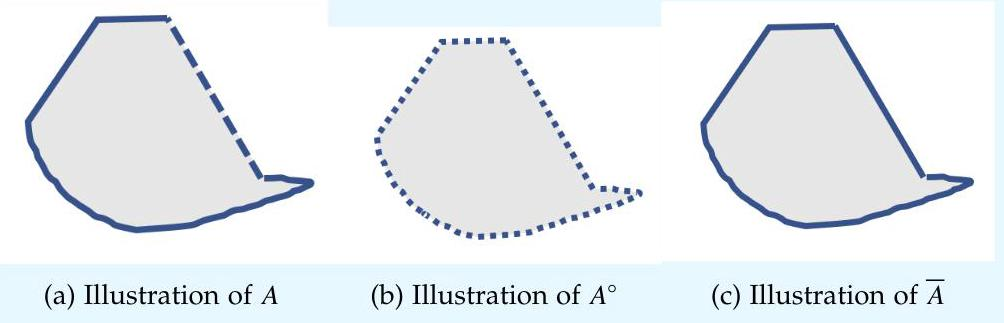
\includegraphics[max width=0.8\textwidth]{images/bo_d2bcsrref24c73avs720_25_282_922_1004_323_0.jpg}
\end{center}
\hspace*{3em} 

Figure 2.1: Graph Illustrations

\begin{itemize}
\item Example 2.10 1. For \(\lbrack a,b) \subseteq  \mathbb{R}\) , we have:
\end{itemize}

\[
\lbrack a,b{)}^{ \circ  } = \left( {a,b}\right) ,\;\overline{\lbrack a,b)} = \left\lbrack  {a,b}\right\rbrack
\]

2. For \(X = \mathbb{R},{\mathbb{Q}}^{ \circ  } = \varnothing\) and \(\overline{\mathbb{Q}} = \mathbb{R}\) .

3. Consider the discrete topology \(\left( {X,{\mathcal{T}}_{\text{ discrete }}}\right)\) , we have

\[
{S}^{ \circ  } = S,\;\bar{S} = S
\]

The insights behind the definition (2.5) is as follows

Proposition 2.10 1. \({A}^{ \circ  }\) is the largest open subset of \(X\) contained in \(A\) ;

\(\bar{A}\) is the smallest closed subset of \(X\) containing \(A\) .

2. If \(A \subseteq  B\) , then \({A}^{ \circ  } \subseteq  B\) and \(\bar{A} \subseteq  \bar{B}\)

3. \(A\) is open in \(X\) is equivalent to say \({A}^{ \circ  } = A;A\) is closed in \(X\) is equivalent to say \(\bar{A} = A\) .

\begin{itemize}
\item Example 2.11 Let(X, d)be a metric space. What’s the closure of an open ball \({B}_{r}\left( x\right)\) ? The direct intuition is to define the closed ball
\end{itemize}

\[
{\bar{B}}_{r}\left( x\right)  = \{ y \in  X \mid  d\left( {x,y}\right)  \leq  r\} .
\]

Question: is \({\bar{B}}_{r}\left( x\right)  = \overline{{B}_{r}\left( x\right) }\) ?

1. Since \({\bar{B}}_{r}\left( x\right)\) is a closed subset of \(X\) , and \({B}_{r}\left( x\right)  \subseteq  {\bar{B}}_{r}\left( x\right)\) , we imply that

\[
\overline{{B}_{r}\left( x\right) } \subseteq  {\bar{B}}_{r}\left( x\right)
\]

2. Howover, we may find an example such that \(\overline{{B}_{r}\left( x\right) }\) is a proper subset of \({\bar{B}}_{r}\left( x\right)\) : Consider the discrete metric space \(\left( {X,{d}_{\text{ discrete }}}\right)\) and for \(\forall x \in  X\) ,

\[
{B}_{1}\left( x\right)  = \{ x\}  \Rightarrow  \overline{{B}_{1}\left( x\right) } = \{ x\} ,\;{\bar{B}}_{1}\left( x\right)  = X
\]

The equality \({\bar{B}}_{r}\left( x\right)  = \overline{{B}_{r}\left( x\right) }\) holds when(X, d)is a normed space. Here is another characterization of \(\bar{A}\) : Proposition 2.11

\[
\bar{A} = \{ x \in  X \mid  \forall \text{ open }U \ni  x,U\bigcap A \neq  \varnothing \}
\]

Proof. Define

\[
S = \{ x \in  X \mid  \forall \text{ open }U \ni  x,U \cap  A \neq  \varnothing \}
\]

It suffices to show that \(\bar{A} = S\) . 1. First show that \(S\) is closed:

\[
X \smallsetminus  S = \left\{  {x \in  X\mid \exists {U}_{x} \ni  x\text{ open s.t. }{U}_{x} \cap  A = \varnothing }\right\}
\]

Take \(x \in  X \smallsetminus  S\) , we imply there exists open \({U}_{x} \ni  x\) such that \({U}_{x} \cap  A = \varnothing\) . We claim

\({U}_{x} \subseteq  X \smallsetminus  S\)

\begin{itemize}
\item For \(\forall y \in  {U}_{x}\) , note that \({U}_{x} \ni  y\) that is open, such that \({U}_{x} \cap  A = \varnothing\) . Therefore,
\end{itemize}

\(y \in  X \smallsetminus  S\) .

Therefore, we have \(x \in  {U}_{x} \subseteq  X \smallsetminus  S\) for any \(\forall x \in  X \smallsetminus  S\) .

Note that

\[
X \smallsetminus  S = \mathop{\bigcup }\limits_{{x \in  X \smallsetminus  S}}\{ x\}  \subseteq  \mathop{\bigcup }\limits_{{x \in  X \smallsetminus  S}}{U}_{x} \subseteq  X \smallsetminus  S,
\]

which implies \(X \smallsetminus  S = \mathop{\bigcup }\limits_{{x \in  X \smallsetminus  S}}{U}_{x}\) is open, i.e., \(S\) is closed in \(X\) .

2. By definition, it is clear that \(A \subseteq  S\) :

\[
\forall a \in  A,\forall \text{ open }U \ni  a,U\bigcap A \supseteq  \{ a\}  \neq  \varnothing  \Rightarrow  a \in  S.
\]

Therefore, \(\bar{A} \subseteq  \bar{S} = S\) .

3. Suppose on the contrary that there exists \(y \in  S \smallsetminus  \bar{A}\) .

Since \(y \notin  \bar{A}\) , by definition, there exists \(F \supseteq  A\) closed such that \(y \notin  F\) .

Therefore, \(y \in  X \smallsetminus  F\) that is open, and

\[
\left( {X \smallsetminus  F}\right) \bigcap A \subseteq  \left( {X \smallsetminus  A}\right) \bigcap A = \varnothing  \Rightarrow  y \notin  S,
\]

which is a contradiction. Therefore, \(S = \bar{A}\) .

Definition 2.6 [accumulation point] Let \(A \subseteq  X\) be a subset in a topological space. We call \(x \in  X\) are an accumulation point (limit point) of \(A\) if

\[
\forall U \subseteq  X\text{ open s.t. }U \ni  x,\left( {U\smallsetminus \{ x\} }\right) \bigcap A \neq  \varnothing .
\]

Proposition \({2.12}\;\bar{A} = A\bigcup {A}^{\prime }\) .

Proof. This proposition directly follows from Proposition (2.11) and the definition of \({\mathrm{A}}^{\prime }\) .

\section*{2.6. Wednesday for MAT4002}

Reviewing.

1. Interior, Closure:

\[
\bar{A} = \{ x \mid  \forall U \ni  x\text{ open },U\bigcap A \neq  \varnothing \}
\]

2. Accumulation points

\section*{2.6.1. Remark on Closure}

Definition 2.14 [Sequential Closure] Let \({A}_{S}\) be the set of limits of any convergent sequence in \(A\) , then \({A}_{S}\) is called the sequential closure of \(A\) .

Definition 2.15 [Accumulation/Cluster Points] The set of accumulation (limit) points is defined as

\[
{A}^{\prime } = \{ x \mid  \forall U \ni  x\text{ open },\left( {U\smallsetminus \{ x\} }\right) \bigcap A \neq  \varnothing \}
\]

®

1. (a) There exists some point in \(A\) but not in \({A}^{\prime }\) :

\[
A = \{ 1,2,3,\ldots ,n,\ldots \}
\]

Then any point in \(A\) is not in \({A}^{\prime }\)

(b) There also exists some point in \({A}^{\prime }\) but not in \(A\) :

\[
A = \left\{  {\left. \frac{1}{n}\right| \;n \geq  1}\right\}
\]

Then the point 0 is in \({A}^{\prime }\) but not in \(A\) .

2. The closure \(\bar{A} = A \cup  {A}^{\prime }\) .

3. The size of the sequentical closure \({A}_{S}\) is between \(A\) and \(\bar{A}\) , i.e., \(A \subseteq  {A}_{S} \subseteq  \bar{A}\) : It’s clear that \(A \subseteq  {A}_{S}\) , since the sequence \(\left\{  {{a}_{n} \mathrel{\text{ := }} a}\right\}\) is convergent to \(a\) for

\(\forall a \in  A\) .

For all \(a \in  {A}_{S}\) , we have \(\left\{  {a}_{n}\right\}   \rightarrow  a\) . Then for any open \(U \ni  a\) , there exists

\(N\) such that \(\left\{  {{a}_{N},{a}_{N + 1},\ldots }\right\}   \subseteq  U \cap  A \neq  \varnothing\) . Therefore, \(a \in  \bar{A}\) , i.e., \({A}_{S} \subseteq  \bar{A}\) .

Question: Is \({A}_{S} = \bar{A}\) ?

Proposition 2.21 Let(X, d)be a metric space, then \({A}_{S} = \bar{A}\) .

Proof. Let \(a \in  \bar{A}\) , then there exists \({a}_{n} \in  {B}_{1/n}\left( a\right)  \cap  A\) , which implies \(\left\{  {a}_{n}\right\}   \rightarrow  a\) , i.e., \(a \in\)  \({A}_{S}\) .

If(X, T)is metrizable, then \({A}_{S} = \bar{A}\) . The same goes for first countable topological spaces. However, \({A}_{S}\) is a proper subset of \(\bar{A}\) in general:

Let \(A \subseteq  X\) be the set of continuous functions, where \(X = {\mathbb{R}}^{\mathbb{R}}\) denotes the set of all real-valued functions on \(\mathbb{R}\) , with the topology of pointwise convergence.

Then \({A}_{S} = {B}_{1}\) , the set of all functions of first Baire-Category on \(\mathbb{R}\) ; and \({\left\lbrack  {A}_{S}\right\rbrack  }_{S} = {B}_{2}\) , the set of all functions of second Baire-Category on \(\mathbb{R}\) . Since \({B}_{1} \neq  {B}_{2}\) , we have \({\left\lbrack  {A}_{S}\right\rbrack  }_{S} = {A}_{S}\) . Note that \(\overline{\bar{A}} = \bar{A}\) . We conclude that \({A}_{S}\) cannot equal to \(\bar{A}\) , since the sequential closure operator cannot be idemotenet.

Definition 2.16 [Boundary] The boundary of \(\mathbf{A}\) is defined as

\[
\partial \mathbf{A} = \bar{A} \smallsetminus  {A}^{ \circ  }
\]

Proposition 2.22 Let(X, T)be a topological space with \(A,B \subseteq  X\) .

\[
\overline{X \smallsetminus  A} = X \smallsetminus  {A}^{ \circ  },\;{\left( X \smallsetminus  B\right) }^{ \circ  } = X \smallsetminus  \bar{B}\;\partial A = \bar{A} \cap  \left( \overline{X \smallsetminus  A}\right)
\]

Proof.

\[
X \smallsetminus  {A}^{ \circ  } = X \smallsetminus  \left( {\mathop{\bigcup }\limits_{{U\text{ is open, }U \subseteq  A}}U}\right)  \tag{2.2a}
\]

\[
= \mathop{\bigcap }\limits_{{U\text{ is open, }U \subseteq  A}}\left( {X \smallsetminus  U}\right)  \tag{2.2b}
\]

\[
= \mathop{\bigcap }\limits_{{V\text{ is closed, }F \supseteq  X \smallsetminus  A}}F \tag{2.2c}
\]

\[
= \overline{X \smallsetminus  A} \tag{2.2d}
\]

Denoting \(X \smallsetminus  A\) by \(B\) , we obtain:

\[
{\left( X \smallsetminus  B\right) }^{ \circ  } = {A}^{ \circ  } \tag{2.3a}
\]

\[
= X \smallsetminus  \left( {X \smallsetminus  {A}^{ \circ  }}\right)  \tag{2.3b}
\]

\[
= X \smallsetminus  \overline{X \smallsetminus  A} \tag{2.3c}
\]

\[
= X \smallsetminus  \bar{B} \tag{2.3d}
\]

By definition of \(\partial A\) ,

\[
\partial A = \bar{A} \smallsetminus  {A}^{ \circ  } \tag{2.4a}
\]

\[
= \bar{A}\bigcap \left( {X \smallsetminus  {A}^{ \circ  }}\right)  \tag{2.4b}
\]

\[
= \bar{A}\bigcap \left( \overline{X \smallsetminus  A}\right)  \tag{2.4c}
\]

\section*{2.6.2. Functions on Topological Space}

Definition 2.17 [Continuous] Let \(f : \left( {X,{\mathcal{T}}_{X}}\right)  \rightarrow  \left( {Y,{\mathcal{T}}_{Y}}\right)\) be a map. Then the function \(f\) is continuous, if

\[
U \in  {\mathcal{T}}_{Y} \Rightarrow  {f}^{-1}\left( U\right)  \in  {\mathcal{T}}_{X}
\]

1. The identity map id : \(\left( {X,\mathcal{T}}\right)  \rightarrow  \left( {X,\mathcal{T}}\right)\) defined as \(x \mapsto  x\) is continuous

2. The identity map id : \(\left( {X,{\mathcal{T}}_{\text{ discrete }}}\right)  \rightarrow  \left( {X,{\mathcal{T}}_{\text{ indiscrete }}}\right)\) defined as \(x \mapsto  x\) is continuous. Since \({\operatorname{id}}^{-1}\left( \varnothing \right)  = \varnothing\) and \({\operatorname{id}}^{-1}\left( X\right)  = X\)

3. The identity map id : \(\left( {X,{\mathcal{T}}_{\text{ indiscrete }}}\right)  \rightarrow  \left( {X,{\mathcal{T}}_{\text{ discrete }}}\right)\) defined as \(x \mapsto  x\) is not continuous.

Proposition 2.23 If \(f : X \rightarrow  Y\) , and \(g : Y \rightarrow  Z\) be continuous, then \(g \circ  f\) is continuous

Proof. For given \(U \in  {\mathcal{T}}_{Z}\) , we imply

\[
{g}^{-1}\left( U\right)  \in  {\mathcal{T}}_{Y} \Rightarrow  {f}^{-1}\left( {{g}^{-1}\left( U\right) }\right)  \in  {\mathcal{T}}_{X},
\]

i.e., \({\left( g \circ  f\right) }^{-1}\left( U\right)  \in  {\mathcal{T}}_{X}\)

Proposition 2.24 Suppose \(f : X \rightarrow  Y\) is continuous between two topological spaces. Then \(\left\{  {x}_{n}\right\}   \rightarrow  x\) implies \(\left\{  {f\left( {x}_{n}\right) }\right\}   \rightarrow  f\left( x\right)\) .

Proof. Take open \(U \ni  f\left( x\right)\) , which implies \({f}^{-1}\left( U\right)  \ni  x\) . Since \({f}^{-1}\left( U\right)\) is open, we imply there exists \(N\) such that

\[
\left\{  {{x}_{n} \mid  n \geq  N}\right\}   \subseteq  {f}^{-1}\left( U\right)
\]

i.e., \(\left\{  {f\left( {x}_{n}\right)  \mid  n \geq  N}\right\}   \subseteq  U\)

We use the notion of Homeomorphism to describe the equivalence between two topological spaces.

Definition 2.18 [Homeomorphism] A homeomorphism between spaces topological spaces \(\left( {X,{\mathcal{T}}_{X}}\right)\) and \(\left( {Y,{\mathcal{T}}_{Y}}\right)\) is a bijection

\[
f : \left( {X,{\mathcal{T}}_{X}}\right)  \rightarrow  \left( {Y,{\mathcal{T}}_{Y}}\right)
\]

such that both \(f\) and \({f}^{-1}\) are continuous.

\section*{2.6.3. Subspace Topology}

Definition 2.19 Let \(A \subseteq  X\) be a non-empty set. The subspace topology of \(A\) is defined as:

1. \({\mathcal{T}}_{A} \mathrel{\text{ := }} \left\{  {U \cap  A \mid  U \in  {\mathcal{T}}_{A}}\right\}\)

2. The coarsest topology on \(A\) such that the inclusion map

\[
i : \left( {A,{\mathcal{T}}_{A}}\right)  \rightarrow  \left( {X,{\mathcal{T}}_{X}}\right) ,\;i\left( x\right)  = x
\]

is continuous.

(We say the topology \({\mathcal{T}}_{1}\) is coarser than \({\mathcal{T}}_{2}\) , or \({\mathcal{T}}_{2}\) is finer than \({\mathcal{T}}_{1}\) , if \({\mathcal{T}}_{1} \subseteq  {\mathcal{T}}_{2}\)

e.g., \({\mathcal{T}}_{\text{ discrete }}\) is the finest topology, and \({\mathcal{T}}_{\text{ indiscrete }}\) is coarsest topology.)

3. The (unique) topology such that for any \(\left( {Y,{\mathcal{T}}_{Y}}\right)\) ,

\[
f : \left( {Y,{\mathcal{T}}_{Y}}\right)  \rightarrow  \left( {A,{\mathcal{T}}_{A}}\right)
\]

is continuous iff \(i \circ  f : \left( {Y,{\mathcal{T}}_{Y}}\right)  \rightarrow  \left( {X,{\mathcal{T}}_{X}}\right)\) (where \(i\) is the inclusion map) is continuous.

Proposition 2.25 The definition (1) and (2) in (2.19) are equivalent.

Outline. The proof is by applying

\[
{i}^{-1}\left( S\right)  = S\bigcap A,\;\forall S
\]

\begin{itemize}
\item Example 2.17 Let all English and numerical letters be subset of \({\mathbb{R}}^{2}\) : P, 6
\end{itemize}

The homeomorphism can be constrcuted between these two English letters.

Proposition 2.26 The definition (2) and (3) in (2.19) are equivalent.

Proof. Necessity.

\begin{itemize}
\item For \(\forall U \in  {\mathcal{T}}_{X}\) , consider that
\end{itemize}

\[
{\left( i \circ  f\right) }^{-1}\left( U\right)  = {f}^{-1}\left( {{i}^{-1}\left( U\right) }\right)  = {f}^{-1}\left( {U \cap  A}\right)
\]

since \(U \cap  A \in  {\mathcal{T}}_{A}\) and \(f\) is continuous, we imply \({\left( i \circ  f\right) }^{-1}\left( U\right)  \in  {\mathcal{T}}_{Y}\)

\begin{itemize}
\item For \(\forall {U}^{\prime } \in  {\mathcal{T}}_{A}\) , we have \({U}^{\prime } = U \cap  A\) for some \(U \in  {\mathcal{T}}_{X}\) . Therefore,
\end{itemize}

\[
{f}^{-1}\left( {U}^{\prime }\right)  = {f}^{-1}\left( {U \cap  A}\right)  = {f}^{-1}\left( {{i}^{-1}\left( U\right) }\right)  = {\left( i \circ  f\right) }^{-1}\left( U\right)  \in  {\mathcal{T}}_{Y}.
\]

The sufficiency is left as exercise.

Proposition 2.27 1. The definition (1) in (2.19) does define a topology of \(A\)

2. Closed sets of \(A\) under subspace topology are of the form \(V \cap  A\) , where \(V\) is closed in \(X\)

Proposition 2.28 Suppose \(\left( {A,{\mathcal{T}}_{A}}\right)  \subseteq  \left( {X,{\mathcal{T}}_{X}}\right)\) is a subspace topology, and \(B \subseteq  A \subseteq  X\) . Then

1. \({\bar{B}}^{A} = {\bar{B}}^{X} \cap  A\) .

2. \({B}^{\circ A} \supseteq  {B}^{\circ X}\)

Proof. By proposition (2.27), \({\bar{B}}^{X} \cap  A\) is closed in \(A\) , and \({\bar{B}}^{X} \cap  A \supset  B\) , which implies

\[
{\bar{B}}^{A} \subseteq  {\bar{B}}^{X}\bigcap A
\]

Note that \({\bar{B}}^{A} \supset  B\) is closed in \(A\) , which implies \({\bar{B}}^{A} = V \cap  A \subseteq  V\) , where \(V\) is closed in \(X\) . Therefore,

\[
{\bar{B}}^{X} \subseteq  V \Rightarrow  {\bar{B}}^{X} \cap  A \subseteq  V \cap  A = {\bar{B}}^{A}
\]

Therefore, \({\bar{B}}^{A} = {\bar{B}}^{X} \subseteq  V\)

Can we have \({B}^{\circ X} = {B}^{\circ A}\) ?

\section*{2.6.4. Basis (Base) of a topology}

Roughly speaking, a basis of a topology is a family of "generators" of the topology.

Definition 2.20 Let(X, T)be a topological space. A family of subsets \(\mathcal{B}\) in \(X\) is a basis for \(\mathcal{T}\) if

1. \(\mathcal{B} \subseteq  \mathcal{T}\) , i.e., everything in \(\mathcal{B}\) is open

2. Every \(U \in  \mathcal{T}\) can be written as union of elements in \(\mathcal{B}\) .

\begin{itemize}
\item Example 2.18 1. \(\mathcal{B} = \mathcal{T}\) is a basis.
\end{itemize}

2. For \(X = {\mathbb{R}}^{n}\) ,

\[
\mathcal{B} = \left\{  {{B}_{r}\left( \mathbf{x}\right)  \mid  \mathbf{x} \in  {\mathbb{Q}}^{n},r \in  \mathbb{Q}\bigcap \left( {0,\infty }\right) }\right\}
\]

Exercise: every \(\left( {a,b}\right)  = \mathop{\bigcup }\limits_{{i \in  I}}\left( {{p}_{i},{q}_{i}}\right)\) for \({p}_{i},{q}_{i} \in  \mathbb{Q}\) .

Therefore, \(\mathcal{B}\) is countable.

Proposition 2.29 If(X, T)has a countable basis, e.g., \({\mathbb{R}}^{n}\) , then(X, T)has a second-countable space.

\section*{3.3. Monday for MAT4002}

\section*{3.3.1. Remarks on Basis and Homeomorphism}

Reviewing.

1. \(A \subseteq  {A}_{S} \subseteq  \bar{A}\) , where \({A}_{S}\) is sequential closure and \(\bar{A}\) denotes closure.

2. Subspace topology.

3. Homeomorphism. Consider the mapping \(f : X \rightarrow  Y\) with the topogical space

\(X,Y\) shown below, with the standard topology, the question is whether \(f\) is continuous?

\begin{center}
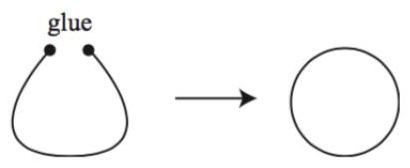
\includegraphics[max width=0.3\textwidth]{images/bo_d2bcsrref24c73avs720_36_777_903_410_168_0.jpg}
\end{center}
\hspace*{3em} 

Figure 3.1: Diagram for mapping \(f\)

The answer is no, since the left in (3.1) can be isomorphically mapped into(0,1); the right can be isomorphically mapped into \(\left\lbrack  {0,1}\right\rbrack\) , and the mapping \(\left( {0,1}\right)  \rightarrow  \left\lbrack  {0,1}\right\rbrack\) cannot be isomorphism:

Proof. Assume otherwise the mapping \(g : \left( {0,1}\right)  \rightarrow  \left\lbrack  {0,1}\right\rbrack\) is isomorphism, and therefore \({f}^{-1}\left( U\right)\) is open for any open set \(U\) in the space \(\left\lbrack  {0,1}\right\rbrack\) .

Construct \(U = (1 - \delta ,1\rbrack\) for \(\delta  \leq  1\) , and therfore \({f}^{-1}(\left( {1 - \delta ,1\rbrack }\right)\) is open, and therfore for the point \(x = {f}^{-1}\left( 1\right)\) , there exists \(\varepsilon  > 0\) such that

\[
{B}_{\varepsilon }\left( x\right)  \subseteq  {f}^{-1}(\left( {1 - \delta ,1\rbrack }\right)  \Rightarrow  \left\lbrack  {x - \varepsilon ,x) \subseteq  {f}^{-1}\left( \left( {1 - \delta ,1}\right) \right) \text{ , and }(x,x + \varepsilon }\right\rbrack   \subseteq  {f}^{-1}\left( \left( {1 - \delta ,1}\right) \right) \text{ . }
\]

which implies that there exists \(a,b\) such that \(\left\lbrack  {x - \varepsilon ,x}\right)  = {f}^{-1}\left( \left( {a,1}\right) \right)\) and \((x,x + \varepsilon \rbrack  =\)  \({f}^{-1}\left( \left( {b,1}\right) \right)\) , i.e., \({f}^{-1}\left( {\left( {a,b}\right)  \cap  \left( {b,1}\right) }\right)\) admits into two values in \(\lbrack x - \varepsilon ,x)\) and \((x,x + \varepsilon \rbrack\) , which is a contradiction.

4. Basis of a topology \(\mathcal{B} \subseteq  \left( {X,\mathcal{T}}\right)\) is a collection of open sets in the space such that the whole space can be recovered, or equivalently

(a) \(\mathcal{B} \subseteq  \mathcal{T}\)

(b) Every set in \(\mathcal{T}\) can expressed as a union of sets in \(\mathcal{B}\)

Example: Let \({\mathbb{R}}^{n}\) be equipped with usual topology, then

\[
B = \left\{  {{B}_{q}\left( x\right)  \mid  x \in  {\mathbb{Q}}^{n},q \in  {\mathbb{Q}}^{ + }}\right\}  \text{ is a basis of }{\mathbb{R}}^{n}\text{ . }
\]

It suffices to show \(U \subseteq  {\mathbb{R}}^{n}\) can be written as

\[
U = {U}_{x \in  \mathbb{Q}}{B}_{{q}_{x}}\left( x\right)
\]

Proposition 3.4 Let \(X,Y\) be topological spaces, and \(\mathcal{B}\) a basis for topology on \(Y\) . Then

\[
f : X \rightarrow  Y\text{ is continuous } \Leftrightarrow  {f}^{-1}\left( B\right) \text{ is open in }\mathrm{X},\forall B \in  \mathcal{B}
\]

Therefore checking \({f}^{-1}\left( U\right)\) is open for all \(U \in  {\mathcal{T}}_{Y}\) suffices to checking \({f}^{-1}\left( N\right)\) is open for all \(B \in  \mathcal{B}\) .

Proof. The forward direction follows from the fact \(B \subseteq  {\mathcal{T}}_{Y}\) .

To show the reverse direction, let \(U \in  {\mathcal{T}}_{Y}\) , then \(U = \mathop{\bigcup }\limits_{{i \in  I}}{B}_{i}\) , where \({B}_{i} \in  \mathcal{B}\) , which implies

\[
{f}^{-1}\left( U\right)  = {f}^{-1}\left( {\mathop{\bigcup }\limits_{{i \in  I}}{B}_{i}}\right)  = \mathop{\bigcup }\limits_{{i \in  I}}{f}^{-1}\left( {B}_{i}\right)
\]

which is open in \(X\) by our hypothesis.

Corollary 3.1 Let \(f : X \rightarrow  Y\) be a bijection. Suppose there is a basis \({\mathcal{B}}_{X}\) of \({\mathcal{T}}_{X}\) such that \(\left\{  {f\left( B\right)  \mid  B \in  {\mathcal{B}}_{X}}\right\}\) forms a basis of \({\mathcal{T}}_{Y}\) . Then \(X \cong  Y\) .

Proof. Suppose \(W \in  {\mathcal{T}}_{Y}\) , then by our hypothesis,

\[
W = \mathop{\bigcup }\limits_{{i \in  I}}f\left( {B}_{i}\right) ,{B}_{i} \in  {\mathcal{B}}_{X} \Rightarrow  {f}^{-1}\left( W\right)  = \mathop{\bigcup }\limits_{{i \in  I}}{B}_{i} \in  {\mathcal{T}}_{X},
\]

which implies \(f\) is continuous.

Suppose \(U \in  {\mathcal{T}}_{X}\) , then

\[
U = \mathop{\bigcup }\limits_{{i \in  I}}{B}_{i} \Rightarrow  f\left( U\right)  = \mathop{\bigcup }\limits_{{i \in  I}}f\left( {B}_{i}\right)  \in  {\mathcal{T}}_{Y} \Rightarrow  {\left\lbrack  {f}^{-1}\right\rbrack  }^{-1}\left( U\right)  \in  {\mathcal{T}}_{Y},
\]

i.e., \({f}^{-1}\) is continuous.

Question: how to recognise whether a family of subsets is a basis for some given topology?

Proposition 3.5 Let \(X\) be a set, \(\mathcal{B}\) is a collection of subsets satisfying

1. \(X\) is a union of sets in \(\mathcal{B}\) , i.e., every \(x \in  X\) lies in some \({B}_{x} \in  \mathcal{B}\)

2. The intersection \({B}_{1} \cap  {B}_{2}\) for \(\forall {B}_{1},{B}_{2} \in  \mathcal{B}\) is a union of sets in \(\mathcal{B}\) , i.e., for each \({B}_{1},{B}_{2} \in  \mathcal{B}\) , and \(x \in  {B}_{1} \cap  {B}_{2}\) , then there exists \({B}_{3} \in  \mathcal{B}\) such that \(x \in  {B}_{3} \subseteq  {B}_{1} \cap  {B}_{2}\) .

Then the collection of subsets \({\mathcal{T}}_{\mathcal{B}}\) , formed by taking any union of sets in \(\mathcal{B}\) , is a topology, and \(\mathcal{B}\) is a basis for \({\mathcal{T}}_{B}\) .

Proof. 1. \(0 \in  {\mathcal{T}}_{\mathcal{B}}\) (taking nothing from \(\mathcal{B}\) ); for \(x \in  X,{B}_{x} \in  \mathcal{B}\) , by hypothesis (1),

\[
X = \mathop{\bigcup }\limits_{{x \in  X}}{B}_{x} \in  {\mathcal{T}}_{\mathcal{B}}
\]

2. Suppose \({T}_{1},{T}_{2} \in  {\mathcal{T}}_{\mathcal{B}}\) . Let \(x \in  {T}_{1} \cap  {T}_{2}\) , where \({T}_{i}\) is a union of subsets in \(\mathcal{B}\) . Therefore,

\[
\left\{  \begin{array}{ll} x \in  {B}_{1} \subseteq  {T}_{1}, & {B}_{1} \in  \mathcal{B} \\  x \in  {B}_{2} \subseteq  {T}_{2}, & {B}_{2} \in  \mathcal{B} \end{array}\right.
\]

which implies \(x \in  {B}_{1} \cap  {B}_{2}\) , i.e., \(x \in  {B}_{x} \subseteq  {B}_{1} \cap  {B}_{2}\) for some \({B}_{x} \in  \mathcal{B}\) . Therefore,

\[
\mathop{\bigcup }\limits_{{x \in  {B}_{1} \cap  {B}_{2}}}\{ x\}  \subseteq  \mathop{\bigcup }\limits_{{x \in  {B}_{1} \cap  {B}_{2}}}{B}_{x} \subseteq  {B}_{1} \cap  {B}_{2}
\]

i.e., \({B}_{1} \cap  {B}_{2} = \mathop{\bigcup }\limits_{{x \in  {B}_{1} \cap  {B}_{2}}}{B}_{x}\) , i.e., \({B}_{1} \cap  {B}_{2} \in  {\mathcal{T}}_{\mathcal{B}}\) .

3. The property that \({\mathcal{T}}_{\mathcal{B}}\) is closed under union operations can be checked directly.

The proof is complete.

\section*{3.3.2. Product Space}

Now we discuss how to construct new topological spaces out of given ones is by taking Cartesian products:

Definition 3.4 Let \(\left( {X,{\mathcal{T}}_{X}}\right) ,\left( {Y,{\mathcal{T}}_{Y}}\right)\) be topological spaces. Consider the family of subsets in \(X \times  Y\) :

\[
{\mathcal{B}}_{X \times  Y} = \left\{  {U \times  V \mid  U \in  {\mathcal{T}}_{X},V \in  {\mathcal{T}}_{y}}\right\}
\]

This \({\mathcal{B}}_{X \times  Y}\) forms a basis of a topology on \(X \times  Y\) . The induced topology from \({\mathcal{B}}_{X \times  Y}\) is called product topology.

For example, for \(X = \mathbb{R},Y = \mathbb{R}\) , the elements in \({\mathcal{B}}_{X \times  Y}\) are rectangles.

Proof for well-definedness in definition (3.4). We apply proposition (3.5) to check whether \({B}_{X \times  Y}\) forms a basis:

1. For any \(\left( {x,y}\right)  \in  X \times  Y\) , we imply \(x \in  X,y \in  Y\) . Note that \(X \in  {\mathcal{T}}_{X},Y \in  {\mathcal{T}}_{Y}\) , we imply \(\left( {x,y}\right)  \in  X \times  Y \in  {\mathcal{B}}_{X \times  Y}\) .

2. Suppose \({U}_{1} \times  {V}_{1},{U}_{2} \times  {V}_{2} \in  {\mathcal{B}}_{X \times  Y}\) , then

\[
\left( {{U}_{1} \times  {V}_{1}}\right)  \cap  \left( {{U}_{2} \times  {V}_{2}}\right)  = \left( {{U}_{1} \cap  {U}_{2}}\right)  \times  \left( {{V}_{1} \cap  {V}_{2}}\right) ,
\]

where \({U}_{1} \cap  {U}_{2} \in  {\mathcal{T}}_{X},{V}_{1} \cap  {V}_{2} \in  {\mathcal{T}}_{Y}\) . Therefore, \(\left( {{U}_{1} \times  {V}_{1}}\right)  \cap  \left( {{U}_{2} \times  {V}_{2}}\right)  \in  {\mathcal{B}}_{X \times  Y}\) .

However, the product topology may not necessarily become the largest topology in the space \(X \times  Y\) . Consider \(X = \mathbb{R},Y = \mathbb{R}\) , the open set in the space \(X \times  Y\) may not necessarily be rectangles. However, all elements in \({\mathcal{B}}_{X \times  Y}\) are rectangles.

\begin{itemize}
\item Example 3.8 The space \(\mathbb{R} \times  \mathbb{R}\) is homeomorphic to \({\mathbb{R}}^{2}\) , where the product topology is defined on \(\mathbb{R} \times  \mathbb{R}\) and the standard topology is defined on \({\mathbb{R}}^{2}\) :
\end{itemize}

Construct the function \(f : \mathbb{R} \times  \mathbb{R} \rightarrow  {\mathbb{R}}^{2}\) with \(\left( {a,b}\right)  \rightarrow  \left( {a,b}\right)\) .

Obviously, \(f : \mathbb{R} \times  \mathbb{R} \rightarrow  {\mathbb{R}}^{2}\) is a bijection.

Take the basis of the topology on \(\mathbb{R}\) as open intervals,

\[
{B}_{X} = \{ \left( {a,b}\right)  \mid  a < b\text{ in }\mathbb{R}\}
\]

Therefore, one can verify that the set \(\mathcal{B} \mathrel{\text{ := }} \{ \left( {a,b}\right)  \times  \left( {c,d}\right)  \mid  a < b,c < d\}\) forms a basis for the product topology, and

\[
\{ f\left( B\right)  \mid  B \in  \mathcal{B}\}  = \{ \left( {a,b}\right)  \times  \left( {c,d}\right)  \mid  a < b,c < d\}
\]

forms a basis of the usual topology in \({\mathbb{R}}^{2}\) .

By Corollary (3.1), we imply \(\mathbb{R} \times  \mathbb{R} \cong  {\mathbb{R}}^{2}\) .

We also raise an example on the homeomorphism related to product spaces:

\begin{itemize}
\item Example 3.9 Let \({S}^{1} = \{ \left( {\cos x,\sin x \mid  x \in  \left\lbrack  {0,{2\pi }}\right\rbrack  }\right) \}\) be a unit circle on \({\mathbb{R}}^{2}\) .
\end{itemize}

Consider \(f : {S}^{1} \times  \left( {0,\infty }\right)  \rightarrow  {\mathbb{R}}^{2} \smallsetminus  \{ \mathbf{0}\}\) defined as

\[
f\left( {\cos x,\sin x,r}\right)  \mapsto  \left( {r\cos x,r\sin x}\right)
\]

It’s clear that \(f\) is a bijection, and \(f\) is continuous. Moreover, the inverse \(g \mathrel{\text{ := }} {f}^{-1}\) is defined as

\[
g\left( {a,b}\right)  = \left( {\frac{a}{\sqrt{{a}^{2} + {b}^{2}}},\frac{b}{\sqrt{{a}^{2} + {b}^{2}}},\sqrt{{a}^{2} + {b}^{2}}}\right)
\]

which is continuous as well. Therefore, the \(f : {\mathcal{S}}^{1} \times  \left( {0,\infty }\right)  \rightarrow  {\mathbb{R}}^{2} \smallsetminus  \{ \mathbf{0}\}\) is a homeomorphism.

\section*{3.6. Wednesday for MAT4002}

\section*{3.6.1. Remarks on product space}

Reviewing.

\begin{itemize}
\item Product Topology: For topological space \(\left( {X,{\mathcal{T}}_{X}}\right)\) and(Y, Y), define the basis
\end{itemize}

\[
{\mathcal{B}}_{X \times  Y} = \left\{  {U \times  V \mid  U \in  {\mathcal{T}}_{X},V \in  {\mathcal{T}}_{Y}}\right\}
\]

and the family of union of subsets in \({\mathcal{B}}_{X \times  Y}\) forms a product topology.

Proposition 3.9 a ring torus is homeomorphic to the Cartesian product of two circles, say \({S}^{1} \times  {S}^{1} \cong  T\) .

Proof. Define a mapping \(f : \left\lbrack  {0,{2\pi }}\right\rbrack   \times  \left\lbrack  {0,{2\pi }}\right\rbrack   \rightarrow  T\) as

\[
f\left( {\theta ,\phi }\right)  = \left( {\left( {R + r\cos \theta }\right) \cos \phi ,\;\left( {R + r\cos \theta }\right) \sin \phi ,\;r\sin \theta }\right)
\]

Define \(i : T \rightarrow  {\mathbb{R}}^{3}\) , we imply

\[
i \circ  f : \left\lbrack  {0,{2\pi }}\right\rbrack   \times  \left\lbrack  {0,{2\pi }}\right\rbrack   \rightarrow  {\mathbb{R}}^{3}\text{ is continuous }
\]

Therefore we imply \(f : \left\lbrack  {0,{2\pi }}\right\rbrack   \times  \left\lbrack  {0,{2\pi }}\right\rbrack   \rightarrow  T\) is continuous. Together with the condition

that

\[
\left\{  \begin{array}{l} f\left( {0,y}\right)  = f\left( {{2\pi },y}\right) \\  f\left( {x,0}\right)  = f\left( {x,{2\pi }}\right)  \end{array}\right.
\]

we imply the function \(f : {S}^{1} \times  {S}^{1} \rightarrow  T\) is continuous. We can also show it is bijective. We can also show \({f}^{-1}\) is continuous.

Proposition 3.10 1. Let \(X \times  Y\) be endowed with product topology. The projection

mappings defined as

\[
{p}_{X} : X \times  Y \rightarrow  X\text{ , with }{p}_{X}\left( {x,y}\right)  = x
\]

\[
{p}_{Y} : X \times  Y \rightarrow  Y\text{ , with }{p}_{Y}\left( {x,y}\right)  = y
\]

are continuous.

2. (an equivalent definition for product topology) The product topology is the coarest topology on \(X \times  Y\) such that \({p}_{X}\) and \({p}_{Y}\) are both continuous.

3. (an equivalent definition for product topology) Let \(Z\) be a topological space, then the product topology is the unique topology that the red and the blue line in the diagram commutes:

\begin{center}
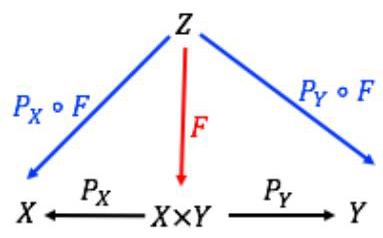
\includegraphics[max width=0.3\textwidth]{images/bo_d2bcsrref24c73avs720_42_640_1003_383_238_0.jpg}
\end{center}
\hspace*{3em} 

Figure 3.3: Diagram summarizing the statement (*)

namely,

the mapping \(F : Z \rightarrow  X \times  Y\) is continuous iff both \({P}_{X} \circ  F : Z \rightarrow  X\) and

\({P}_{Y} \circ  F : Z \rightarrow  Y\) are continuous. (*)

Proof. 1. For any open \(U\) , we imply \({p}_{X}^{-1}\left( U\right)  = U \times  Y \in  {\mathcal{B}}_{X \times  Y} \subseteq  {\mathcal{T}}_{X \times  Y}\) , i.e., \({p}_{X}^{-1}\left( U\right)\) is open. The same goes for \({p}_{Y}\) .

2. It suffices to show any topology \(\mathcal{T}\) that meets the condition in (2) must contain \({\mathcal{T}}_{\text{ product }}\) . We imply that for \(\forall U \in  {\mathcal{T}}_{X},V \in  {\mathcal{T}}_{Y}\) ,

\[
\left\{  {\begin{array}{l} {p}_{X}^{-1}\left( U\right)  = U \times  X \in  \mathcal{T} \\  {p}_{Y}^{-1}\left( V\right)  = X \times  V \in  \mathcal{T} \end{array} \Rightarrow  \left( {U \times  Y}\right)  \cap  \left( {X \times  V}\right)  = \left( {U \cap  X}\right)  \times  \left( {Y \cap  V}\right)  = U \times  V \in  \mathcal{T},}\right.
\]

which implies \({\mathcal{B}}_{X \times  Y} \subseteq  \mathcal{T}\) . Since \(\mathcal{T}\) is closed for union operation on subsets, we

imply \({\mathcal{T}}_{\text{ product topology }} \subseteq  \mathcal{T}\) .

3. (a) Firstly show that \({\mathcal{T}}_{\text{ product }}\) satisfies (*).

\begin{itemize}
\item For the forward direction, by (1) we imply both \({p}_{X} \circ  F\) and \({p}_{Y} \circ  F\) are continuous, since the composition of continuous functions are continuous as well.
\end{itemize}

\begin{itemize}
\item For the reverse direction, for \(\forall U \times  {\mathcal{T}}_{X},V \in  {\mathcal{T}}_{Y}\) ,
\end{itemize}

\[
{F}^{-1}\left( {U \times  V}\right)  = {\left( {p}_{X} \circ  F\right) }^{-1}\left( X\right)  \cap  {\left( {p}_{Y} \circ  F\right) }^{-1}\left( Y\right) ,
\]

which is open due to the continuity of \({p}_{X} \circ  F\) and \({p}_{Y} \circ  F\) .

(b) Then we show the uniqueness of \({\mathcal{T}}_{\text{ product }}\) . Let \(\mathcal{T}\) be another topology \(X \times  Y\) satisfying (*).

\begin{itemize}
\item Take \(Z = \left( {X \times  Y,\mathcal{T}}\right)\) , and consider the identity mapping \(F = \mathrm{{id}} : Z \rightarrow  Z\) , which is continuous. Therefore \({p}_{X} \circ  \mathrm{{id}}\) and \({p}_{Y} \circ  \mathrm{{id}}\) are continuous, i.e., \({p}_{X}\) and \({p}_{Y}\) are continuous. By (2) we imply \({\mathcal{T}}_{\text{ product }} \subseteq  \mathcal{T}\) .
\end{itemize}

\begin{itemize}
\item Take \(Z = \left( {X \times  Y,{\mathcal{T}}_{\text{ product }}}\right)\) , and consider the identity mapping \(F = \mathrm{{id}}\) : \(Z \rightarrow  Z\) . Note that \({p}_{X} \circ  F = {p}_{X}\) and \({p}_{Y} \circ  F = {p}_{Y}\) , which is continuous by (1). Therefore, the identity mapping \(F : \left( {X \times  Y,{\mathcal{T}}_{\text{ product }}}\right)  \rightarrow  \left( {X \times  Y,\mathcal{T}}\right)\) is continuous, which implies
\end{itemize}

\[
U = {\operatorname{id}}^{-1}\left( U\right)  \subseteq  {\mathcal{T}}_{\text{ product }}\text{ for }\forall U \in  \mathcal{T}\text{ , }
\]

i.e., \(\mathcal{T} \subseteq  {\mathcal{T}}_{\text{ product }}\) .

The proof is complete.

Definition 3.6 [Disjoint Union] Let \(X \times  Y\) be two topological spaces, then the disjoint union of \(X\) and \(Y\) is

\[
X\coprod Y \mathrel{\text{ := }} \left( {X\times \{ 0\} }\right)  \cup  \left( {Y\times \{ 1\} }\right)
\]

1. We define that \(U\) is open in \(X \coprod  Y\) if

(a) \(U \cap  \left( {X\times \{ 0\} }\right)\) is open in \(X \times  \{ 0\}\) ; and

(b) \(U \cap  \left( {Y\times \{ 1\} }\right)\) is open in \(Y \times  \{ 1\}\) .

We also need to show the well-definedness for this definition.

2. \(S\) is open in \(X \coprod  Y\) iff \(S\) can be expressed as

\[
S = \left( {U\times \{ 0\} }\right)  \cup  \left( {V\times \{ 1\} }\right)
\]

where \(U \subseteq  X\) is open and \(V \subseteq  Y\) is open.